% Latex Code by Richard Socher, www.socher.org, permission granted to redistribute, if this line is left here ;)

\documentclass[
%   pdftex,
    a4paper,
    12pt,
%   twoside,
    oneside,
    idxtotoc,
    halfparskip,
%    chapterprefix,
]{scrbook}

\usepackage{moreverb}

%\usepackage{german}
%\usepackage[german]{babel}
%�,�,�,� 
\usepackage[latin1]{inputenc}


\usepackage{longtable}
\usepackage{tabularx}


\usepackage{graphics}

\usepackage{verbatim}

\usepackage{listings}

\usepackage{array}

\usepackage[refpages]{gloss}


\usepackage{amsmath}
\usepackage{amssymb}

\usepackage{courier}

\usepackage{rotating}

\usepackage{color}

\usepackage{comment}

%\definecolor{LinkColor}{rgb}{0,0,0.5} % blue links in pdf?
\definecolor{LinkColor}{rgb}{0,0,0}
\usepackage[%
    pdftitle={Bachelor Thesis},%
    pdfauthor={Richard Socher},%
    pdfcreator={LaTeX with hyperref},
    pdfsubject={Automatic Extension of Feature-based Semantic Lexicons via Bootstrapping Algorithms},
    pdfkeywords={semantic, bootstrapping}]{hyperref}
\hypersetup{colorlinks=true,%
    linkcolor=LinkColor,%
    citecolor=LinkColor,%
    filecolor=LinkColor,%
    menucolor=LinkColor,%
    pagecolor=LinkColor,%
    urlcolor=LinkColor}




\makegloss 
% do this in shell to update:
% directoryOfThesis> bibtex baa_main.gls


\definecolor{lightblue}{rgb}{0.8,0.85,1}
\lstset{backgroundcolor=\color{lightblue}}

\begin{document}

\nocite{*} % The command \nocite{*} causes all items in the database to be included in the references, regardless of whether or not they are cited in the paper.



%\pagenumbering{roman}
%for 1.5 spacing:
%\renewcommand{\baselinestretch}{1.50}\normalsize

%-------------------------------------------------
%- Abstract
%-------------------------------------------------
%\section*{Abstract}

This thesis focuses on game development for Android, an operating system for mobile phones developed by Google. The market for Android applications is currently growing rapidly, and there are currently many games available. The purpose of this thesis is to find out how to develop a competitive Tower Defense game on this expanding market.

Tower Defense is not a new game concept. There are several games of this type with different  themes and gameplay already on the market. In order to provide a solid foundation from which a new Tower Defense game can be developed, many of the existing games were examined thoroughly to find desirable features. In addition to this, interviews with people that play Tower Defense games frequently were conducted, making sure no important features were left out.

The conclusion of the research was that in order to make the game competitive on the Android Market, the gameplay had to be unique. The features of the mobile device were used as tools to achieve this goal. Smartphones primarily provide two features that were taken into consideration when developing Eskimo Tower Defense; the touchscreen and the accelerometer. The touchscreen provides a new interaction method in comparison with similar games on a computer platform. However, this alone did not suffice to distinguish a Tower Defense game on the Android platform. Eskimo Tower Defense utilizes the accelerometer to give players a feeling of being able to control the game, making them more physically involved in the gameplay.
%\newpage

%-------------------------------------------------
%- Table of contents
%-------------------------------------------------
%\tableofcontents

%\newpage

%-------------------------------------------------
%- Vocabulary
%-------------------------------------------------
\section*{Vocabulary}

\emph{\bf{Mob type:}} Each mob type has some unique characteristics. In the current implementation of the game there are four mob types, but more types can be added easily when the game is extended. Some mob types have special abilities; others are only characterized by the values of their standard attributes, such as health or armor. Visually a mob type is recognized by a unique look.

\emph{\bf{Mob wave (or wave):}} A mob wave consists of one or more mobs that will enter the game as a group. All the mobs in the wave are of the same type. The mobs enter the game one by one and walk the path in a line. There is a few seconds between each wave.

\emph{\bf{Tower:}} Towers are built to prevent mobs from reaching the end of the road. A tower can have different types; normal, splash, slow and air. They all have different graphical represenation like brown Eskimo, purple Eskimo, snowman and igloo.

\emph{\bf{Tower level:}} A tower have several upgradable levels. For each level it is getting stronger. 

\emph{\bf{Track:}} A track has a background image, a mob path, a set of mob waves and a current high score. The game has several tracks, which are placed along the progression route on the progression map. To complete a track the player must survive through all mob waves. Each time a mob manages to reach the end of the path without being killed, the player loses one life. If the player's lives reaches zero, the track is lost and the player has to replay it.

\emph{\bf{Track progression map (or progression map):}} The progress map visualizes the player's progress in the game and lets him choose which track he wants to play. The progress map resembles a geographical map where each track is a geographical site placed along a route. The progress map is customized to match the theme of the game. In our implementation it depicts a route from the North Pole to The Sun.

\emph{\bf{Progression route:}} The progression route is a fixed route that dictates in what order the tracks must be completed by the player. The route is visualized on the track progression map. Each track in the game is placed somewhere along the route. To be able to play a certain track the player must first complete any tracks before it. The route may be forked, in which case only one way leading to a track needs to be cleared in order to play that track. The player\'s current progression is visualized with icons.

\emph{\bf{Player:}} The player is the physical person who is playing the game.

\emph{\bf{OpenGL (Open Graphics Library):}} Is a programming interface to write applications with computer graphics. Often used to write 3 dimensional games.  

%-------------------------------------------------
%- Content
%-------------------------------------------------
\newpage
\pagenumbering{arabic}
%-------------------------------------
%- Chapter 1
%-------------------------------------
\chapter{Introduction}

\section{Background}

In the beginning of 2007 a powerful development of smartphones in the mobile phone market was introduced. The introduction of the Iphone by Apple was the starting signal of this rapid development. Since then, several other IT companies have released this type of phone. Most of these smartphones have operating systems from Symbian, RIM, Apple, Microsoft or Google CITE"(Canalys, 2010)". What they all have in common is that it is relatively simple to develop software for them, meaning that anyone with basic programming skills can develop their own applications. 

Every smartphone operating system has their own system for publishing applications. These applications can be downloaded from users with the same operating system. It is up to the developers to charge a fee for their applications or if they want, give them away for free. This new way of marketing applications allows everyone from bigger companies to the individual developer to compete under the same conditions.

The development of a game was chosen because it consists of a lot of the common obstacles encountered during software development. The difficulties of programming a game include drawing of graphics, managing code efficiency as well as implementing a good system for user interaction. A game is also a good place to start when experimenting with new input methods. The concept of Tower Defense was chosen for the fact that there were few if any Tower Defense games that featured the use of an accelerometer in its game design. 

A Tower Defense is a common type of game often found as Flash-applications on websites. The general concept is that the games feature creatures, organized into waves, that try to go from point A to point B. The objective of the game is to prevent the creatures from reaching their final destination. This is achieved by constructing towers that fire automatically and intermittently upon creatures that enter their range. The game is often varied by introducing different paths creatures can take; some games allow players to construct obstacles that force the mobs to take a certain path, giving the towers additional time to fire. The games often feature different towers with different purposes, as well as different creatures with varying attributes, weaknesses and strengths. 

\section{Purpose and delimitations}

The purpose of this project is to investigate how the new interaction possibilities of smartphones could be used in a real-time game environment. The goal is to develop the basis of a commercially viable game for the android platform that makes use of the touchscreen and accelerometer in new and innovative ways.

The main focus of the project is to develop a stable, extendable and correctly implemented structure for the game, so that further development is facilitated. The number of tracks, tower types, mob types and different sound effects is intentionally small, since focus lies on functionality rather than quantity.
Game balance has a huge impact on commercial viability. If people think the game is unbalanced, they might not want to play it. Due to this fact, one of the goals of this project is to make the game feel as balanced as possible. This can be done by altering values and properties of different game objects, creating synergy and making all elements of the game attractive to the user. The game should be easy to play but still provide a challenge for the user.

Phone model compatibility has not been a main focus. Since the Android platform is designed to provide developers and phone manufacturers with a good foundation on which to base their software, the platform inherently has a good degree of cross-model robustness. However, in order to ensure proper compatibility, the software was tested on three different phone models (HTC Hero, HTC Legend and HTC Desire). Another difference between models is the CPU power and this fact was not taken into consideration during the project. More information on this can be found under ''future work''.
%-------------------------------------
%- Chapter 2
%-------------------------------------
\chapter{Theory}

\section{Android architecture}

Developing for the Android platform is done using the Java programming language. All code can be written using standard approaches of Java programming. However, the Android operating system has very large influence on how applications are executed on the system. Most operating systems on personals computers normally allow the user to run several applications concurrently in different windows, that can also be viewed simultaneously. On the Android device, there is no native way of seeing what applications are running. The hardware buttons on the device are used to either close applications or send them to the background. Since there is no feedback on what happened to the application, it is important to handle such events in a consistent manner.
 
Gaining access to the surface of an Android device requires an implementation of the Activity class. The first describing line in the Android API about activities is ''An activity is a single, focused thing that the user can do'' CITE(Android, 2010). To create an application that shows something to the user, an Activity must be implemented. If it is not important to display information to the user, the Service class may be used (a class that is designed for applications running in the background).

%-------------------
%- Image ACTIVITY DIAGRAM
%-------------------
\begin{figure}[here]
\begin{center}
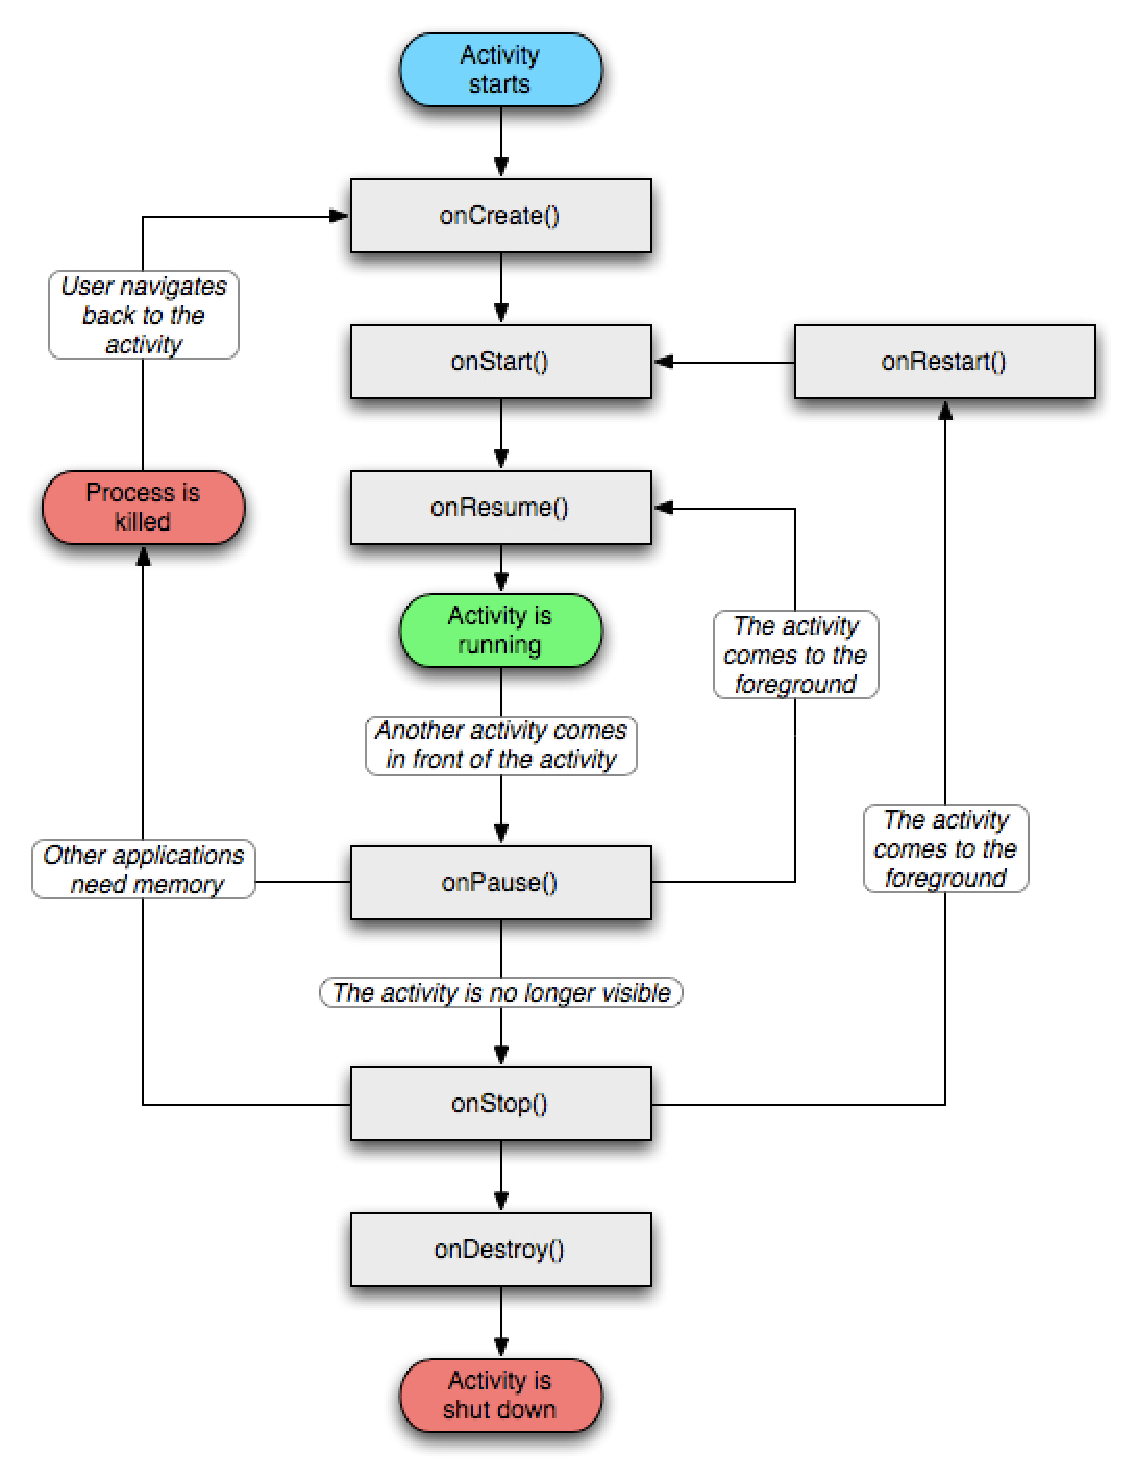
\includegraphics[scale=0.5]{pics/chapters/chapter2/activity_lifecycle2}
\end{center}
\caption{Life cycle of an Activity}
\label{fig:androidActivityLifeCycle}
\end{figure}
%-------------------------------

As can be seen in figure ~\ref{fig:androidActivityLifeCycle}, onCreate(), onStart() and onResume() are all invoked as an activity is first created. Several other methods are also invoked when the operating system needs to manage memory shortage. Once the activity is up and running, it is important to handle these methods correctly. For instance, when a lot of variables are instantiated in the onStart()-method, memory leaks might occur if they are not set to null in the onStop()-method. Memory leaks can cause the entire device to slow down, which can be very frustrating for the user.
 
The graphical layout of an activity consists of objects of the View class. Views can be defined either procedurally while creating the activity, or by accessing predefined layouts from XML-files. In Android applications, views are both responsible for drawing images to the screen and for taking care of events generated from user interaction. For instance, a button is a view that can register listeners for onClick-events. Similarly, events generated by the trackball, hardware buttons and touchscreen are also handled by views.

External resources are often used when developing for Android. Any type of file can be included to the binary files when building an application. If Eclipse is being used to develop the application, a file called R.java is generated whenever the resource directory is updated. This file contains translations from integer resource pointers to variable names that are easier to understand. When the application is built, the resource files are compiled into binary files that load fast and efficiently. \\ CITE (http://developer.android.com/guide/topics/resources/resources-i18n.html)

Accessing resources is done by invoking the method getResources() on the Context that is attached to the application. Context is an interface that is implemented by fundamental Android classes, such as Activity or Service. As stated in the Android API CITE (Android 2010), "It allows access to application-specific resources and classes.".

%----------------------------------------------------------
%----------------------------------------------------------
\subsection{Data storage}

The file system on Android devices differs from systems used on personal computers. On a personal computer, file system data files for one application can be read by any other application. On Android devices however data files created by one application is only readable to that application. Android has four different solutions to store and receive data from the file system on a mobile phone; preferences, files, databases and network. CITE(Android 2010) 

The preferences solution uses key-value pairs to write simple data types, such as texts to be loaded at the start of an application, or settings the user wants to be saved for next time he starts the application. This data is a lightweight method of writing and retrieving data, and is therefor recommended to use for simple data types. CITE(Android 2010)

Another way to manage data storage is to use files. This is a basic way to handle data on the mobile phone's memory card, where files are created, written to and read from. CITE(Android 2010) 

Android also comes with the possibility of using databases for data storage. The type of database available on a Android device is SQLite. CITE(Android 2010) SQLite is a lightweight database engine, built to suit devices with limited memory. It reads and writes to files on the device\'s file system. "A complete SQL database with multiple tables, indices, triggers, and views, is contained in a single disk file." CITE(SQLite 2010)

As long as the phone is connected to the Internet, either via 3G or via a wireless network, it is possible to use the network connection to send and receive data. (Android 2010)
%----------------------------------------------------------
%----------------------------------------------------------
\subsection{Graphics}

There are three approaches to handling graphics when working with Android. The first approach uses predefined layouts in XML-files. The other two approaches involve the Java class Canvas or the cross-language standard specification OpenGL. The Canvas class provides simple tools like rectangles, color filters and bitmaps that let you draw pictures on the screen. It is handled like layers even if it is not exactly layers; the last object that is drawn on the canvas will be drawn on top of anything that was drawn earlier. Canvas only supports two axes, x- and y-coordinates compared to OpenGL that has full support for programming 3D graphics.

For each activity using a predefined layout, there has to be an XML file describing the layout. There is a built-in XML-editor in the Android Software Development Kit for Eclipse that you can use to create these layouts. The editor shows a preview of the window that will be shown on the screen of the device (see figure ~\ref{fig:xmlEditor}). Inside that window is where all the graphics are put. The editor is very easy to use as it uses the drag-and-drop concept. There are several layout options such as GridView, ListView and LinearLayout to choose between and combine. There are also several view options such as normal View, Button, Checkbox, TextView and many more. Items are dragged and dropped to their correct positions. There is also a property window for every item, that gives access to customizing that particular item in the layout. 

%-------------------------
%- IMAGE XML Editor
%-------------------------
\begin{figure}[here]
\begin{center}
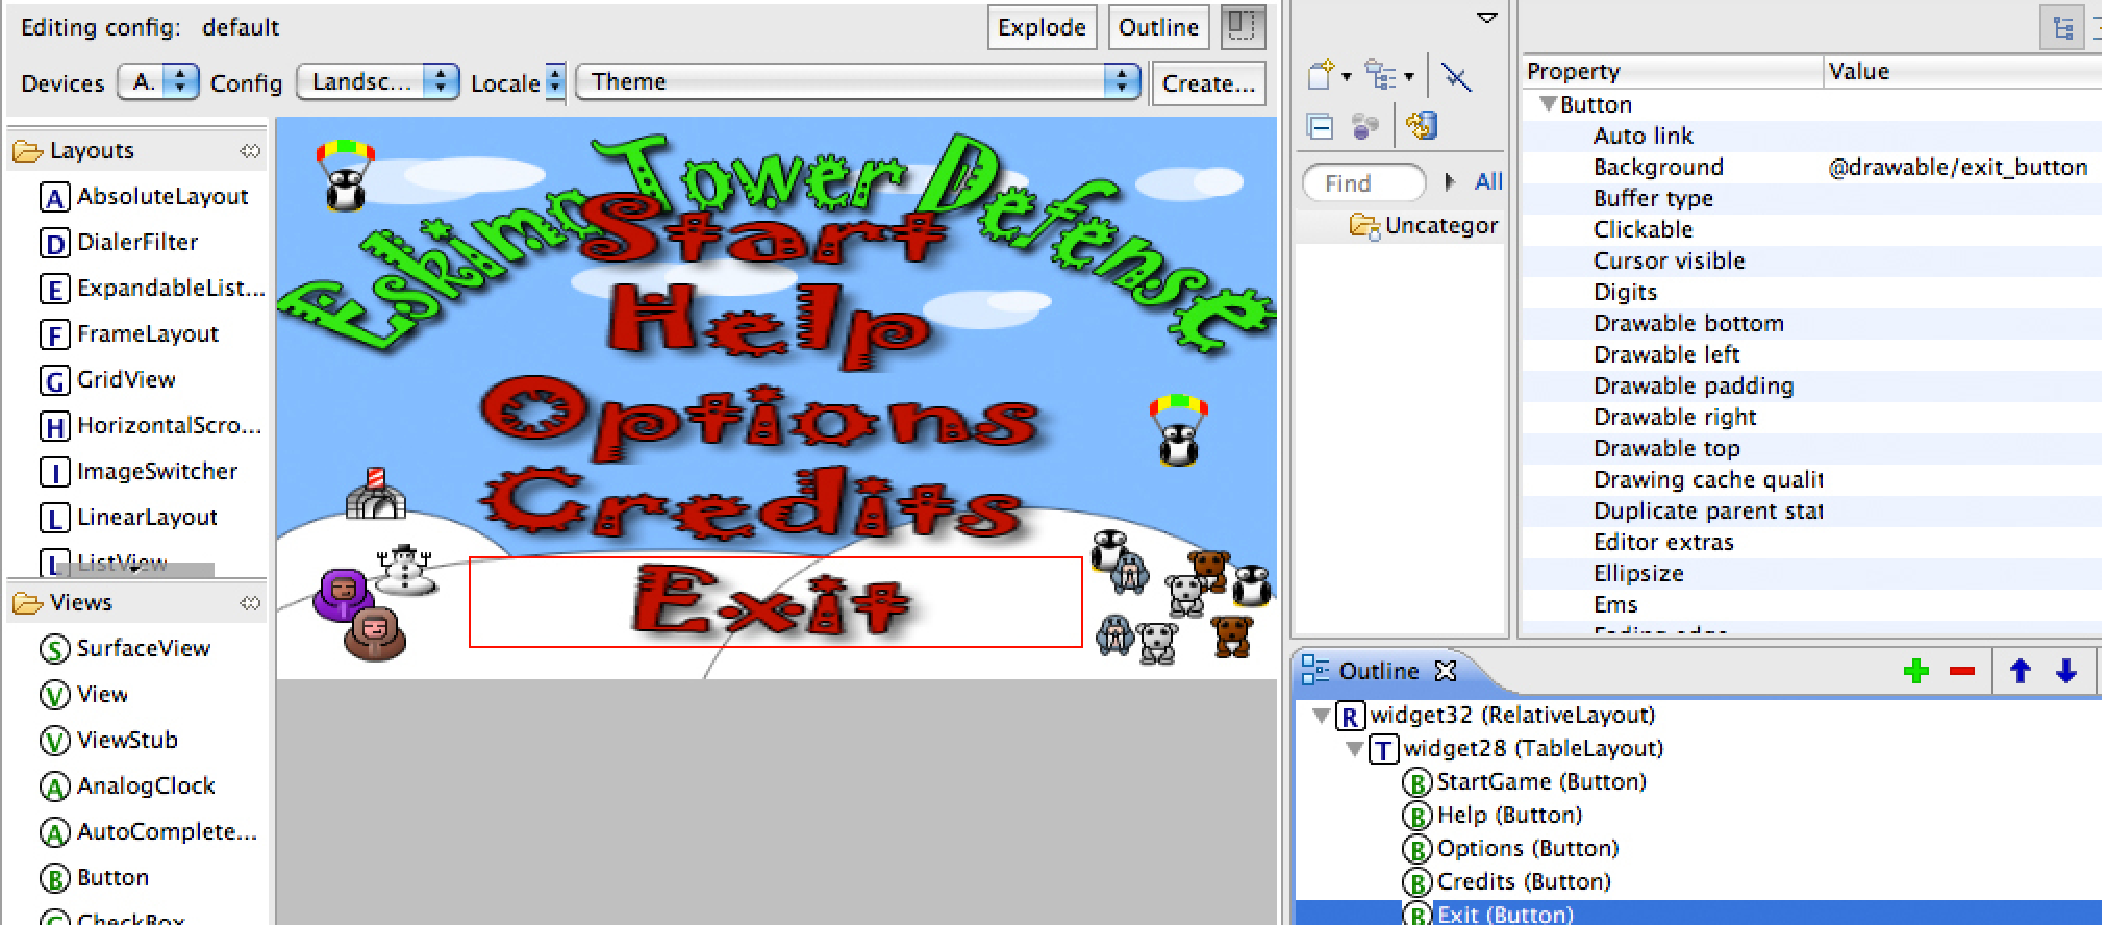
\includegraphics[scale=0.3]{pics/chapters/chapter2/xmleditor}
\end{center}

\caption{Caption for the xmleditor}
\label{fig:xmlEditor}

\end{figure}
%-------------------------

%----------------------------------------------------------
%----------------------------------------------------------
\subsection{Sound}

The Android operating system is able to provide playback of different media files. A list of all supported media formats is published in the Android API (Android 2010). When considering sound files in particular, it is clear that all of the major sound formats are supported (MP3, MIDI, WAVE, Ogg Vorbis and more). Unless playing sounds is the main purpose of the application, it is desirable to use files that are small and do not require lots of memory. 

Implementations of using sound in Android applications are done by utilizing the classes MediaPlayer and SoundPool. The SoundPool class should be used for small sounds, sounds that are likely to be repeated a lot. Properties of this class are described in the Android API (Android 2010). Sounds added to a SoundPool are decoded by a MediaPlayer and stored as raw bitstreams. Not having to decode sound files every time they are played reduces the risk of experiencing performance issues due to heavy CPU load. MediaPlayer is better used for long sound files, such as background music in games. 
%----------------------------------------------------------
%-------------------------------------
%- Chapter 3
%-------------------------------------
\chapter{Method}

Prior to designing the game, background information was collected on developer team's views and expectations on a new Tower Defense game. A number of existing well-known tower defense games were also tested and discussed for research purposes and to get a general idea of what features are desirable. The design process included many discussions of different ideas, drawing of mind maps and sketch-like UML-diagrams.

The development was done in Eclipse IDE with the Android SDK-plugin with the program language Java. Included in Android SDK is an emulator which made it possible to test the code directly on the computer.

The implementation was done using an agile development approach, in the sense that we worked in small iterations and changed the requirements continuously during the development process. To be able to make the project easy to maintain, subversion management with Git was used. This increased our ability to share code within the developer team during the development process, and to allow us to work on multiple parts of the project at the same time. 

%----------------------------------------------------------
\section{Interviews}

Interviews were used as a tool in two different stages of development; the research stage and the final testing stage.

To get a better picture of what makes a Tower Defense game good and try to collecting ideas for the game, interviews were conducted. The interviewees where people that play games regularly and had prior experience of playing Tower Defense games. Ten interviews were conducted, following a unstructured interview template with mainly open questions. The full interview template is found in Appendix APPENDIX"". 

The interviews provided some insight into peoples thoughts and the statements from the participants were used when making important design decisions. It soon became obvious that everyone had their own opinion on which features a good game should include, but several statements were general and helped avoiding common mistakes. 
%----------------------------------------------------------
\section{Git - A version control system}

When developing software in teams, a system to manage and synchronize the source code is needed. This to ensure everyone in the project is working on the latest version of the system. In this project Git was used for this purpose. 

When working with Git each developer included in the project has one local repository on their computer. Changes made to the code is then copied between the other developers local repositories. This does not force the users to have a dedicated server to store a central repository. Instead Git users are free to store their repositories anywhere. (Git, 2010) 

Since Git allows the project to be stored locally on every members computer, work can be done on the implementation despite lack of internet access. This also means that any system failure is only going to affect one individual, who could then fetch an updated version of the project from the other members, providing the project with an increased tolerance to any system breakdowns
%----------------------------------------------------------
\section{Code convention}

Code convention is a huge subject of its own, and it can be divided into subcategories such as style, language and programming practices. When developing a large system it is important to follow a common code style convention. This to make the code easy to understand for other developers that might be working on the system later on. This involves choosing suitable names for variables and classes, as well as making similar choices of code constructions. 

\subsection{Style conventions}

Android is an open source project, and a set of rules have been created to keep a common style between developers. These rules are intended for contributors to the android platform itself. Even though they are not a requirement for application development, they are still well thought out and adapted to the Android environment. For this reason these rules were used as guidelines for this project as well. Some of these could be seen as common sense while others add extra readability beyond what is common in Java programming.

The following are some of the important style conventions that were used, and how they differ from the android contributor rules:

\subsubsection{Javadoc and comments}

Javadoc comments were continuously added to the code, using the standard format as specified in by android. Non-javadoc comments were used as often as well to clearify the code and increase maintainability. A comment including copyright info were not added, since this was deemed to not be needed for the project at this stage.

\subsubsection{Short methods}

Long methods were broken down into shorter ones to increase readability where possible. One good example of this is the method onDraw in the class GameView. This calls several submethods that draws different parts of the game, instead of drawing everything inside one single method.

%--------------------------------
%- Code snippet onDraw
%--------------------------------
\begin{figure}[htb]
\begin{small}
\verbatiminput{code/onDraw.java}
\end{small}
\caption{Caption for onDraw...}
\label{fig:codeExOnDraw}
\end{figure}
%--------------------------------

\subsubsection{Fields}

Fields should either be at the top of the file or immediately before the methods that use them, according to the rules. All fields were declared at the top of the file. Java code conventions recommend field declaration in the following order: "First the public class variables, then the protected, then package level (no access modifier), and then the private." CITE(http://java.sun.com/docs/codeconv/)

\subsubsection{Limit the scope of local variables}

Local variables should be initialized on the same line as they are declared if possible, and also as close as possible to where they are actually used.

\subsubsection{Indentation}

The rules recommend using four spaces instead of tabulations. Since this project was made entirely in Eclipse we chose to use normal tabs. This is the default way to handle indentation when using Eclipse and it is facilitated by using auto-indenting options.

\subsubsection{Field names and other names}

For field names the rules were strictly followed. This means:

%---------------
\begin{itemize}

\item Non-public, non-static field names start with m.
\item Static field names start with s.
\item Other fields start with a lower case letter.
\item Public static final fields (constants) are ALL\_CAPS\_WITH\_UNDERSCORES.

\end{itemize}
%---------------

Additionally field name were carefully chosen so that their purpose was clear, and use of ambiguous names or shortenings was avoided.

\subsubsection{TODO annotation}

The TODO annotation was used extensively during the coding process, to mark unfinished sections in the code. Eclipse automatically recognizes the TODO-comments and makes it even easier for the developer to find them by marking their locations on the scrollbar while browsing the code.

\subsubsection{Logging}

Logging was used for debugging purposes. The log method made it possible to spot sections in the code that was not functional. Debug messages were marked as verbose, meaning that they were only compiled in debug mode. This to ensure that they would not affect the performance of the game.
%----------------------------------------------------------
\section{Android development environment}

Developing standard Android applications requires the Java Development Kit (JDK) and an Integrated Development Environment (IDE). Google recommends Eclipse with Android Development Tools (ADT) for programming applications to Android. The ADT is a plugin for Eclipse allowing easy creation and management of Android projects. CITE HERE""

The Eclipse Foundation is an open-source community originally created by IBM in 2001. Its most popular IDE Package is the Eclipse IDE for Java EE Developers that currently has over 1.2 million downloads. Eclipse IDE is free to use and allows the users to easily create Java applications. (Eclipse Foundation, www.eclipse.org, 2010-04-30)

Figure ~\ref{fig:eclipseIDE} shows a screenshot of a project in Eclipse. The left panel shows all the files in the project and the center panel the current open file. At the bottom there is a console showing the status of the different tasks that Eclipse is performing. To the right is an outline of the methods and variables in the current file. This is generated automatically and helps the user easily overview and navigate the code.

%-------
%- Image eclipse
%-------
\begin{figure}[here]
\begin{center}
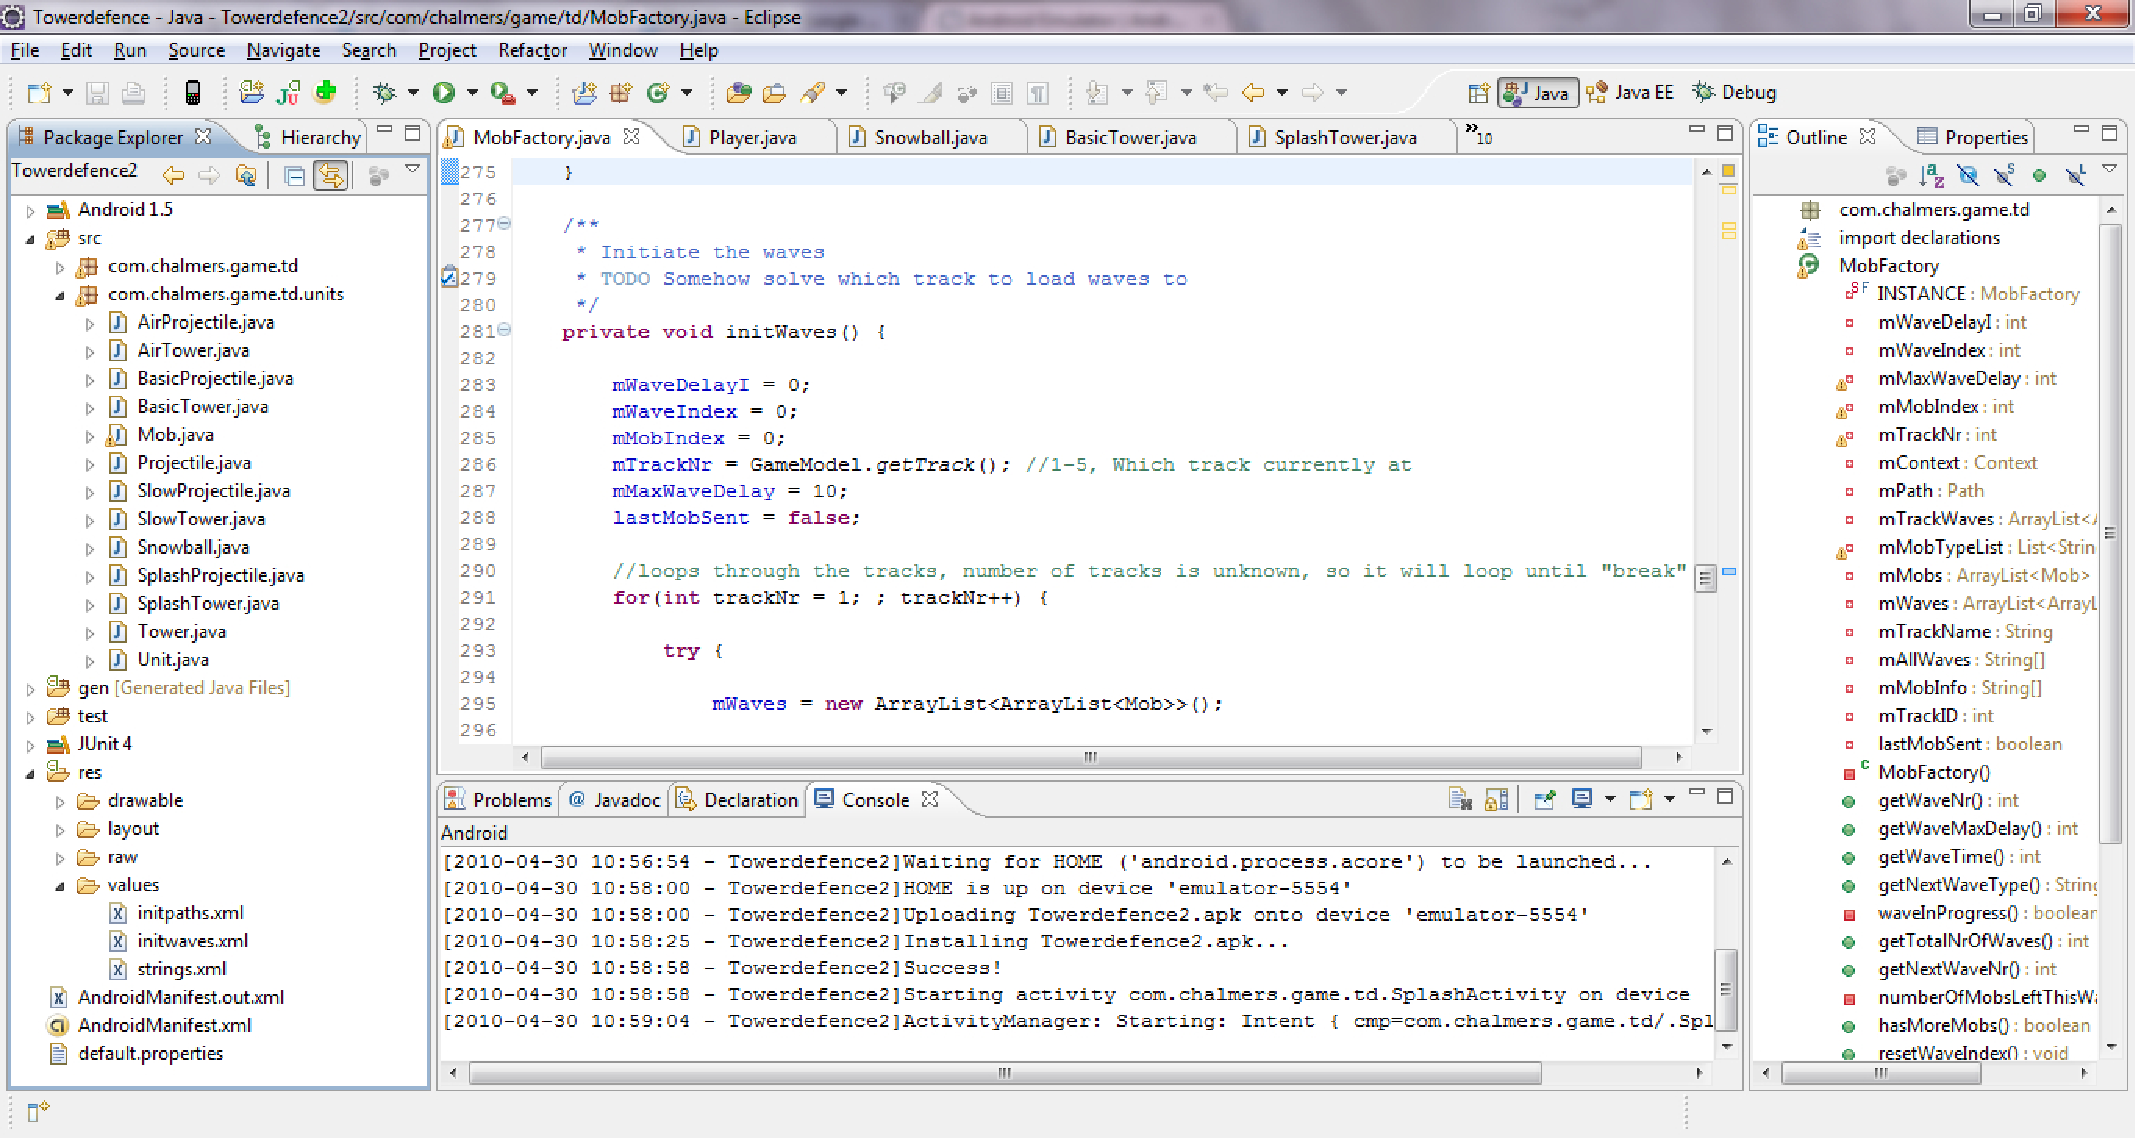
\includegraphics[scale=0.3]{pics/chapters/chapter2/eclipse}
\end{center}
\caption{The eclipse Intergrated Development Environment}
\label{fig:eclipseIDE}
\end{figure}
%-------

The Android Development Kit includes an Android emulator. This allows the developer to test her applications without the use of an actual phone. It supports a majority of the functionalities of a real phone such as simulating SMS, phone calls, events and geographic locations (like GPS navigation). The mouse can be used to click on the screen to emulate usage of the touchscreen of the device. As shown in figure ~\ref{fig:androidEmulator}, there is also access to the buttons normally available on an Android phone. The emulator can be set up to use different versions of Android and different resolutions, allowing the developer to verify compatibility. CITE HERE ""

\clearpage
%-------
%- Image Android emulator
%-------
\begin{figure}[here]
\begin{center}
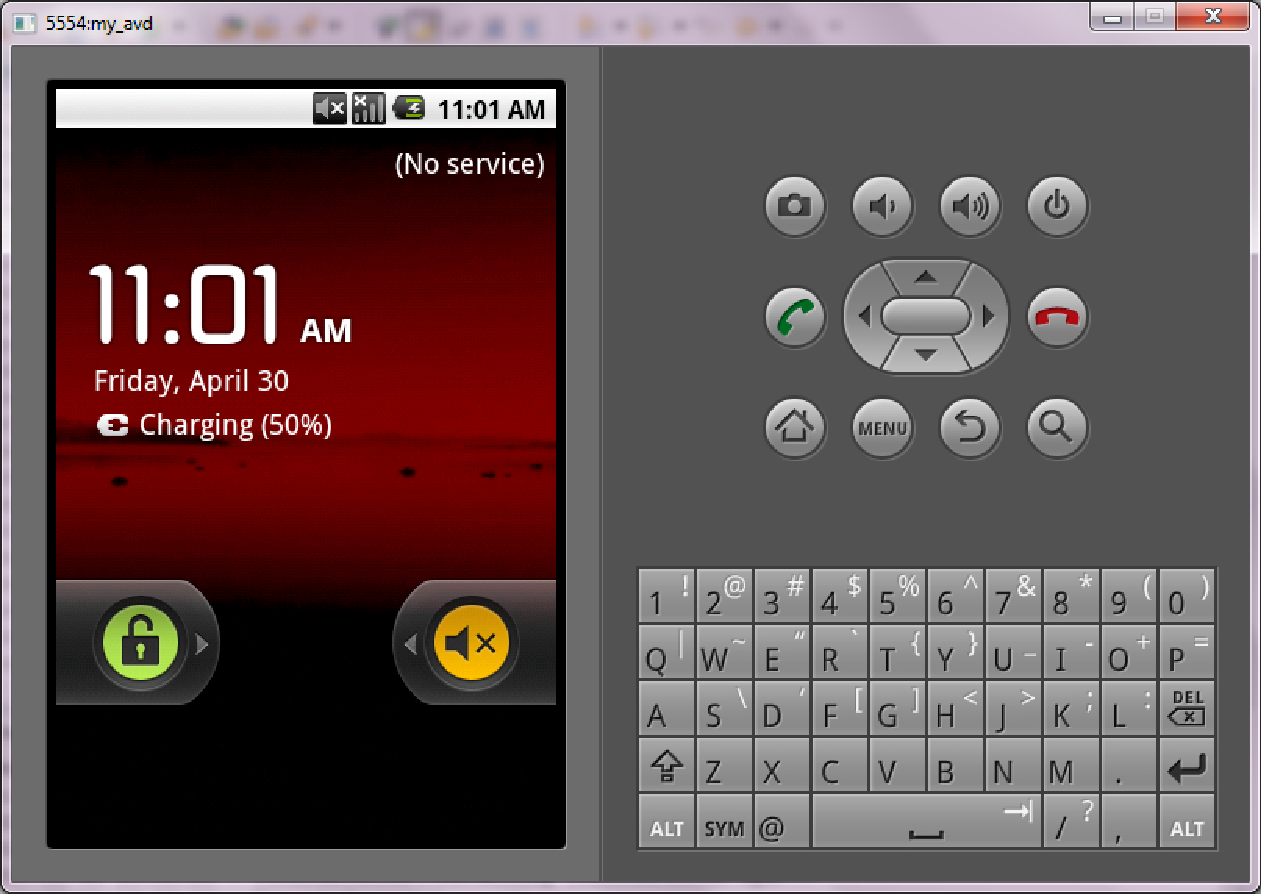
\includegraphics[scale=0.4]{pics/chapters/chapter2/emulator}
\end{center}
\caption{The Android emulator}
\label{fig:androidEmulator}
\end{figure}
%-------
%-------------------------------------
%- Chapter 4
%-------------------------------------
\chapter{Results}

%----------------------------------------------------------
\section{The resulting game: Eskimo Tower Defense}

Text...
%----------------------------------------------------------
%----------------------------------------------------------
\subsection{Structure}
Text...

\subsubsection{UML}

Text...
%----------------------------------------------------------
%----------------------------------------------------------
\subsection{XML layout}

Text...
%----------------------------------------------------------
%----------------------------------------------------------
\subsection{Graphics}

Text...

\subsubsection{Draw}

Text...

\subsubsection{Animation}

Text...

\subsubsection{Menus}
Text...

\subsubsection{Tower placement}

Text...
\subsubsection{Tower upgrade}
Text...
\subsubsection{Mobs}
Text...
%----------------------------------------------------------
%----------------------------------------------------------
\subsection{Progression map}
Text...

%----------------------------------------------------------
%----------------------------------------------------------
\subsection{Tracks}
Text...
%----------------------------------------------------------
%----------------------------------------------------------
\subsection{Physical buttons}
Text...
%----------------------------------------------------------
%----------------------------------------------------------
\subsection{Game play}

Text...
%----------------------------------------------------------
%----------------------------------------------------------
\subsection{Units}

Text...
%----------------------------------------------------------
%----------------------------------------------------------
\subsection{Towers}
Text...
\subsubsection{Subclasses}
Text...
%----------------------------------------------------------
%----------------------------------------------------------
\subsection{Mobs}
Text...
%----------------------------------------------------------
%----------------------------------------------------------
\subsection{Waves}
Text...
%----------------------------------------------------------
%----------------------------------------------------------
\subsection{Path}
Text...
%----------------------------------------------------------
%----------------------------------------------------------
\subsection{Snowball - Accelerometer based interaction}
Text...
%----------------------------------------------------------
%----------------------------------------------------------
\subsection{Projectiles}
Text...

\subsubsection{Subclasses}

Text...
%----------------------------------------------------------
%----------------------------------------------------------
\subsection{Money and high-score}

Text...
%-------------------------------------
%- Chapter 5
%-------------------------------------
\chapter{Discussion}
%----------------------------------------------------------
\section{Design choices}
%----------------------------------------------------------
%----------------------------------------------------------
\subsection{Fixed path versus maze building}

The first important design decision that had to be taken was to decide the movement pattern of the mobs. The Tower Defense genre is divided into two distinctive groups when it comes to mob movement over the map: fixed path or maze building. With a fixed path the mobs move along a pre-defined route on the track and towers can be built along the sides. Maze building games on the other hand, consist of an open field where the mobs can move freely. It is up to the player to build obstacles forcing them to take detours towards the exit. The obstacles that are used are in most cases the towers themselves. 

While testing different games during the research stage of development, one of the tested games was Robo Defence (Lupid Labs, 2010) for Android which featured maze-style gameplay. Robo Defence is one of the most popular Tower Defense games currently on the app-market, distinguishing the game from from this popular alternative was one big factor in deciding upon the fixed path design.

There are many benefits with the fixed path model. Using a fixed path makes the game less complex to the player. It is more forgiving when it comes to the placement of towers: maze building games can get frustrating if the control is imprecise, because a tower in the wrong place might destroy the entire maze. Another benefit is that it gives the level designer more control over the tracks, making it easier to vary track design by varying the path.

Another reason for using the fixed path solution was that none of the team members had much prior experience of game development. For this reason it was decided to keep the complexity at a minimum. The maze building solution would imply the use of artificial intelligence which would be too time consuming, because of the increase in complexity. The static path design seemed to be the least complicated to use when developing a game for the first time. To assure a unique gameplay the focus was instead directed to other implementations, such as the snowball.
%----------------------------------------------------------
%----------------------------------------------------------
\subsection{Theme}

One of the major subjects of discussion in the group was deciding the theme of the game. Since no one in the team had any graphical experience the theme was decided late in the project. At first, placeholders were used to test the functionality of the game. This was later changed to a temporary theme to get started with the graphics. 

It was decided that the game should have a background story that the theme should be linked to. In an early discussion, a green house effect-theme was discussed. The story would then be that animals from the north pole would flee from their melting environment. A map with that story would then have different themes, for instance polluting factories, melting ice caps and smog.

Finally it was decided to use an Eskimo theme. The background story was the same but instead of the green-house effect the animals were migrating south because they desired to move to a warmer climate. The Eskimo tribes frowns upon this since they depend on the wildlife for food and clothing. The tribes therefor set out to prevent this disaster from occuring. The maps will gradually become greener and warmer when progressing throughout the game. The towers were designed as different Eskimos, the snowman and the igloo canon. The mobs became animals such as penguins, polar bears and walruses. In addition to the standard units of a Tower Defense one new special unit is implemented; the snowball. The snowball is a powerful unit which rolls around the screen to run over the mobs as the player tilts the phone.
%----------------------------------------------------------
%----------------------------------------------------------
\subsection{Projectile algorithm}

%- CODE SNIPPET HERE

%----------------------------------------------------------
%----------------------------------------------------------
\subsection{Waves}

A big issue was how the waves were supposed to work. In other Tower Defense games like Bloons and Element Tower Defense the game pauses between every wave, giving time for the user to build more towers. Another way is to make the waves come continuously but with a delay between them. It was decided to use the delay approach. This to ensure that the game flows better and to remove unnecessary actions. Since the tracks feature lot of waves this might be irritating for the player to always have to press a button between each wave.

Since the mobs have varying speed, this may result in having one wave catch up with the previous wave. This is very noticeable during the boss waves. A boss wave consists of one mob with alot more health than a normal mob taking a more considerable effort to kill. Since there only is one mob on boss waves, the countdown until the next wave starts immediately after it is created. To solve this we simply increased the delay after slow boss waves.
%----------------------------------------------------------
\section{Concept}
%----------------------------------------------------------
%----------------------------------------------------------
\subsection{Unique features}

The development of the game called for distinguishing it from other Tower Defense games to make it more desirable for potential customers. Modern Android phones offer many new ways to control applications which could be taken advantage of. The idea was to add an extra dimension to the game using the phones accelerometer. One of the ideas was to control the towers by tilting the phone. Another idea was that the player should be able to control the range of the towers. If the player tilts the phone to the left, the towers range will increase in that direction. Another idea was to control the speed of the mobs. When tilting to the left, it would create a slop to the left making the mobs moving left go faster and mobs moving right slower. 

Studies did not find any other games that has multiple paths for the mobs so this would be an easy feature to implement that would make it more unique. Another thought was letting the user control which way the mobs go in a crossroad using the accelerometer. The more the phone is tilted in one direction, the higher the probability is, that the mobs choose that way.

The idea that was actually implemented was that of a snowball. The snowball will roll over the map controlled by tilting the phone, almost like the classical board game Labyrinth. The player can use this snowball to kill mobs when in difficult situations. Some discussion was had regarding how the snowball would interact with the units on the map. Initially it was designed to kill every mob it touched. This was the easiest way to code it but it made the snowball too good, especially against bosses who had much more health than other mobs. Later, this was changed to dealing damage based on a percentage of the mobs health every frame it touched them. The snowball was also modified to deal less damage to bosses in order to make it more balanced compared to normal mobs. 

There was also a discussion whether the snowball should have any negative aspect to make it harder to use. One idea was to have the snowball not only damage the mobs but also the towers. This combined with a more powerful snowball would make it both effective in hard situations but also a risk. The problem with this is that the player then could place the snowball on the path and without tilting the phone killing the mobs very effective. This would discourage the user from tilting the phone and use the snowball as it was intended. This is also a problem even without the snowball killing the towers but then the snowball would be balanced to take less damage.

%----------------------------------------------------------
%----------------------------------------------------------
\subsection{User interface}

User interface is one of the most important areas when working with touchscreen mobile phones or small touch-screens in general. The small screen needs to hold a lot of information. But,  since the touch-screen is operated with the user\'s fingers, and some people might have bigger fingers than others, it is important that items are not too small. This can make the player irritated when trying to hit the buttons. You do not want to make them too big either which can result in leaving a cluttered interface.  

You want to fit as much as you can but you also want to keep it clean for the user. There were many discussions about which buttons would be the most important for the player during the different states of the game. To keep it clean, pressing a button often brings up a menu with several options to choose from.

The game is played with the screen in landscape position, meaning that most users will only use his thumbs to interact. This means that the buttons must be even bigger compared to if the index finger would have been used.
%----------------------------------------------------------
%----------------------------------------------------------
\subsection{Animations}

Animations was not the main priority during the development. At first, the development was focused on having a working game with innovative features. During testing, it became clear that a game with no animations would be pretty boring. To give the player a good experience the game needed a more realistic feeling. The interviews also revealed that sounds and animations were positive for the game experience. Therefor animations were added to the mobs, which makes them look like they are wobbling back and forth when they are walking down the path. This small change made the game look much more dynamic. There is also an animation at the end of the path where the mobs dive into the water. 
%----------------------------------------------------------
%----------------------------------------------------------
\section{Game balance}

For a game to be interesting and thus sellable, it must provide just enough challange to the user. In strategic games like Tower Defense it is also important that there is room for different types of strategies. Both of these requirements are achieved by balancing the game. This section describes how the different parts of the game were balanced and why.

\subsection{Towers}

Balancing of the towers was done to make sure that no tower was superior to the others. Being able to finish the game by only building one type of tower would make the game boring and unchallenging. The idea was that the player needed to build different towers for different situations. This is one of the reasons for having different types of towers and mobs. Different maps contains different combinations of mob types means the user has to change his strategy to meet the challenges he faces.
%----------------------------------------------------------
%----------------------------------------------------------
\subsection{Mob waves}

The biggest part was balancing of mob waves. Each mob killed awards the player with money. To make the game balanced, the income should be similar to the cost of building towers. If too much money was rewarded the game would not be challenging and if the reward was too small it would be impossible to finish.

Since the maps have different difficulty we had to manually set the health of the waves for each map. The waves of the first map should be easier than the waves of the second map and so on. 
%----------------------------------------------------------
%----------------------------------------------------------
\subsection{Snowball}

The player get one snowball for each 4000 points that is collected. The reason for this amount is that a game normally results in a total of around 10 000 to 15 000 points. This is done to limit the amount of times the user has access to the snowball, and two to three times per map recieved good feedback in testing.

The damage of the snowball was also up for discussion. At first, the snowball killed the mobs instantly. This was later changed to deal damage equal to 8\% of the current health of the mob, each frame. The snowball was also modified to do less damage for each frame it spent on bosses. This because they have around 15 times more health than normal mobs. If the snowball would deal the same amount of damange to the bosses, the snowball would be too powerful.
%----------------------------------------------------------
\section{Insight} %- Temporary headline

Text...
%----------------------------------------------------------
%----------------------------------------------------------
\section{Future work}

The game that resulted from this project is playable in its current state. However, additional features could be added to increase the value of the game. It is also an excellent basis from which a commercial game can be built. This chapter includes several implementations that were thought of but never realized are discussed.

\subsection{Public highscore}

To make the game more attractive and addictive, which was one of the purposes of the project, a public highscore could have been implemented. This would allow the users to play not only to complete the game, but also to compete against others by trying to beat their highscores. A server was needed to be able to upload and store the users scores. This was considered to take too much time and was not that important for the total game experience, therefore not implemented.
%----------------------------------------------------------
%----------------------------------------------------------
\subsection{Fixed frame rate}

If the game was ever to have a public highscore, the game need to be fair. If the game is run faster on phones with faster processors it would not be fair. Then the players with slower phones would have an advantage towards the rest of the players. To solve this the game has to run in the same speed independent of the speed of the phones processor. There is also a problem with future phones with superior processor speed. These phones would run the game so fast it would be very hard for users to play it. There are a number of well-known methods available to achieve this effect. These were excluded from this project in favor of adding features that more directly affect the game experience. This issue is one of the highest prioritised of future work. 
%----------------------------------------------------------
%----------------------------------------------------------
\subsection{Sounds}

In the current version of the game the only sounds included are the background music and a sound effect when the mobs reaches the water. According to our last interviews many people wanted sound effects when the mobs were killed. This would according to them increase the addicting factors of the game. Implementing more sound effects was planed but there was no time to add this for all the situations in the game.
%----------------------------------------------------------
%----------------------------------------------------------
\subsection{Achievments}

Another thing that might increase the game's lifespan is achievements. This is a form of extra bonuses given to the player for completing predetermined tasks. Completing these achievements would unlock new functionalities or new maps. These achievements could be relatively hard to complete. They would also give the user something to strive against after completing all the standard maps in the game.
%----------------------------------------------------------
%----------------------------------------------------------
\subsection{Snowball improvement}

The snowball is one of the main parts that separates us from other Tower Defence games. To further improve the game experience, it is very important that this special weapon is fun and easy to use. If it is not implemented good the player might not use it. He would then miss out of one of the things that makes the game unique. Further development of the snowball is therefore a important part to focus on.

Since the snowball is never introduced properly, new players might not notice it exists. The snowball is one of the more unique parts of the game and it would be very bad if the player never uses it. A message or sound that indicate that the snowball is available would be helpful. The way the snowball is implemented could also be improved. It could for example bounce or even damage towers on the map to make it more challenging to use. The graphics for the snowball could also be improved. Now the snowball is able to roll over the water. One suggestion was that is should be sink or melt faster in the water. Instead of killing the mobs, there was an idea to have the snowball stun the mobs. This would stop them from walking for a moment so the towers had more time to shoot them.
%----------------------------------------------------------
%----------------------------------------------------------
\subsection{More bonus weapons}

One of the unique parts of our game is the snowball which is controlled by the tilt of the phone. An addition to the game could be to extend this idea to more player controllable weapons. A weapon that would daze or stun the mobs momentary was discussed. This could be graphically represented as an earthquake for example.  The idea of a snowball falling down from the sky was also discussed. All these ideas would further make our game more unique and stand out from competition on Android Market.
%-------------------------------------

%- Appendix A - List of figures
% input{chapters/appendixA}

%- Appendix B - UML
% input{chapters/appendixB}


\newpage

\gloss[nocite]{*} \printgloss{glossary}

% command to update:: 
% makeindex -s baa_main.ist -t baa_main.glg -o baa_main.gls baa_main.glo

\newpage

%\chapter{Appendix}
%\addcontentsline{toc}{chapter}{Appendix}
%\appendix

% \chapter{Extra Tables}
% \begin{table}[hbt]
%  \centering
%    \tiny
% \begin{tabularx}{16cm}{|l||X|X|X|X|X|X||X|X|X|X|X|X|X|}
%  \hline
% Characteristic  &Prec. adj   &Prec. obj   &Prec. subj  &Recall adj  &Recall obj  &Recall subj &Prec. 3Same &Prec. 3Same pos.  &Prec. 2Same &Prec. 2Same pos.  &Recall 3Same    &Recall 2Same  \\
% \hline
%human:+     &0.9205 &0.9633 &0.9588 &0.4154 &0.4707 &0.4233 &0.9979 &0.9952 &0.9820 &0.9492 &0.2553 &0.4520 \\
%geogr:-     &0.9406 &0.9525 &0.9382 &0.4825 &0.5098 &0.4704 &0.9907 &0.5000 &0.9744 &0.4176 &0.3446 &0.5010 \\
%spatial:+   &0.8611 &0.9814 &0.9628 &0.3625 &0.4703 &0.4357 &0.9992 &0.9985 &0.9855 &0.9858 &0.2223 &0.4417 \\
%legper:+    &0.9154 &0.9657 &0.9631 &0.4103 &0.4716 &0.4258 &0.9986 &0.9955 &0.9834 &0.9512 &0.2519 &0.4526 \\
%\hline
%sort:d+     &0.8513 &0.9516 &0.9343 &0.3584 &0.4532 &0.4186 &0.9903 &0.9880 &0.9667 &0.9651 &0.2113 &0.4268 \\
%sort:na-    &0.9792 &0.9791 &0.9882 &0.5306 &0.5370 &0.5045 &0.9888 &1.0000 &0.9831 &1.0000 &0.4144 &0.5295 \\
%\hline
%\end{tabularx}
%  \caption{Combining results of the three main relations, parameter combination: 2-5}\label{table.combine3.2-5}
%\end{table}




%\newpage
\addcontentsline{toc}{chapter}{Bibliography}
\bibliographystyle{plain}
\bibliography{references}




\end{document}

 
